\documentclass{article}
\usepackage[utf8]{inputenc}
\usepackage{amsmath, amsfonts, physics}
\newtheorem{definition}{Definition}[section]
\usepackage{graphicx}
\usepackage{minted}

\setminted[python]{breaklines, framesep=2mm, fontsize=\footnotesize, numbersep=5pt}
\graphicspath{ {./practical_images/} }

\title{Singular Value Decomposition: Practical}
\author{1807730}
\date{October 2022}

\begin{document}
	\maketitle
	\newpage
	
	\section{Image Decomposition}
	One practical example of singular value decomposition is in case of an image. For greyscale images we can take the luminosity value at each pixel and use this to construct a matrix representation of the image. In the case of coloured images, each pixel is represented as a tuple of three integers indicating the intensity of the red, green and blue components. Consider figure \ref{fig:test_image}:
	
	\begin{figure}[h]
		\centering
		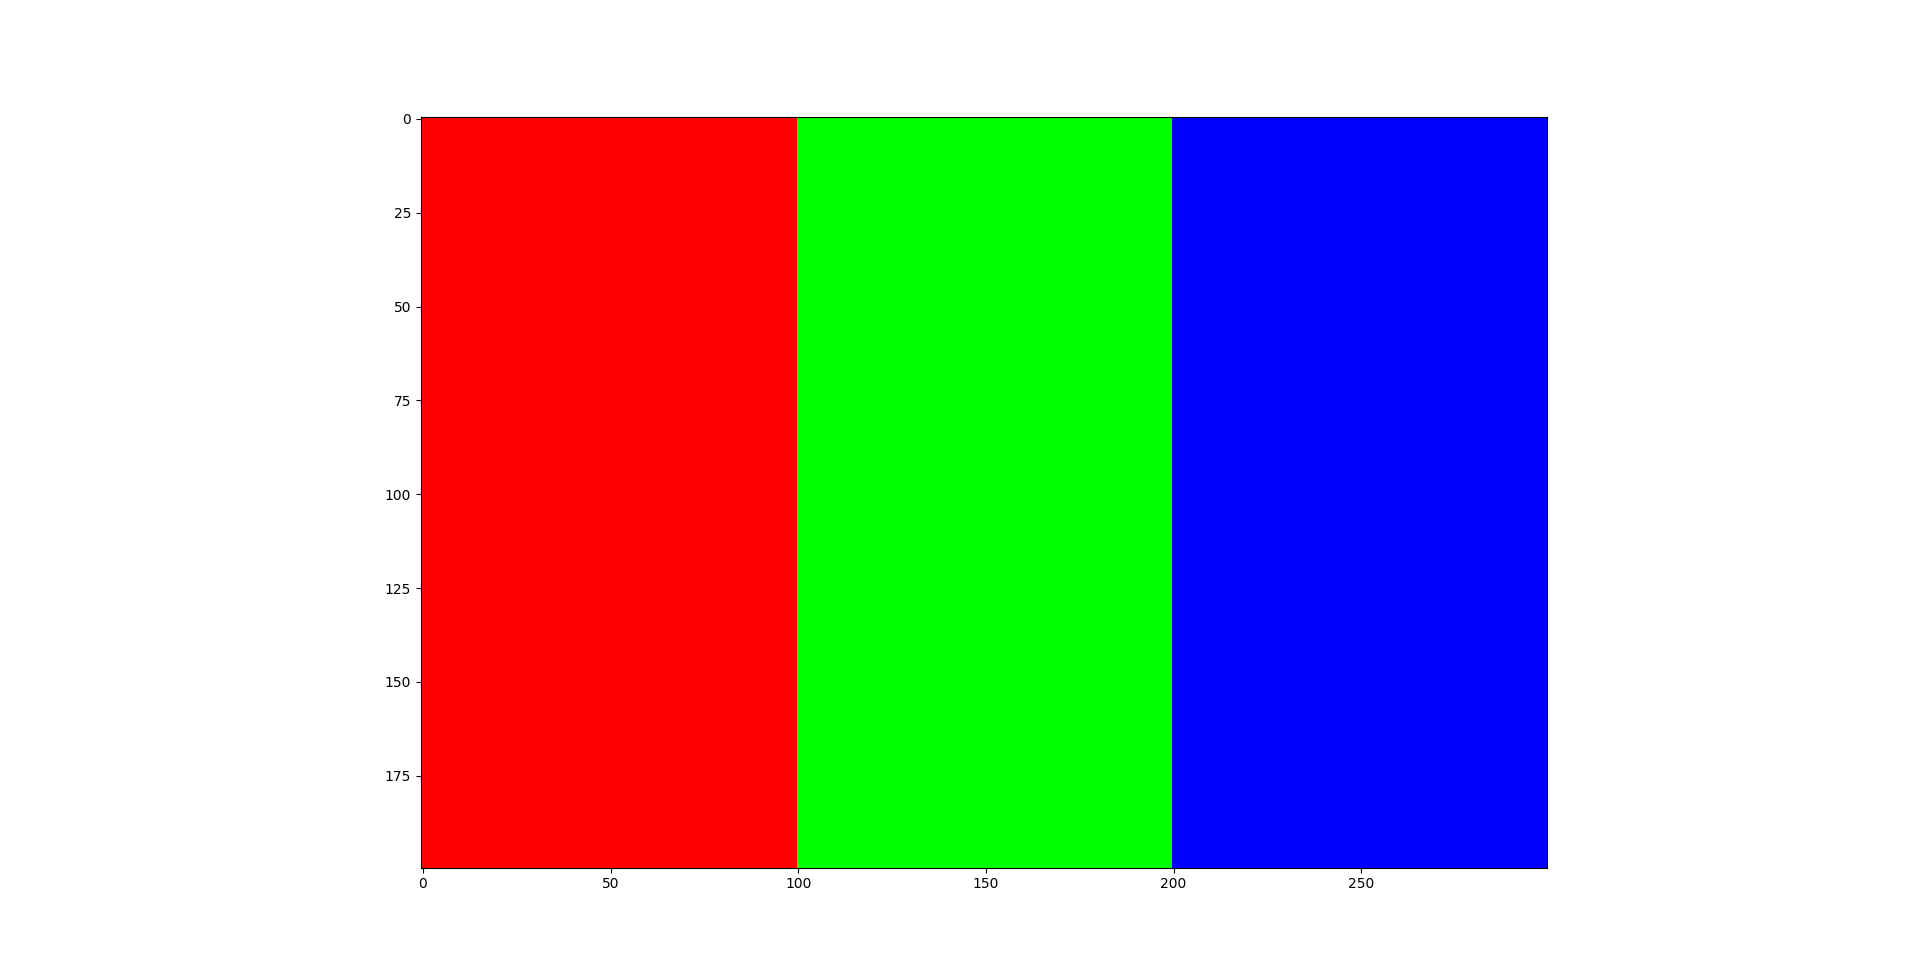
\includegraphics[width=0.4\textwidth]{test_image_plot.png}
		\caption{Test Image for SVD}
		\label{fig:test_image}
	\end{figure}

	This image is $200 \times 300$ in size. It's split into $200 \times 100$ segments with each part taking the maximum intensity of its respective colour. The colour of each pixel in the red section is $(255, 0, 0)$, in the green section it's $(0, 255, 0)$ and the blue section is $(0, 0, 255)$. We can break this image down into three images where each pixel is the intensity of the respective colour:
	
	\begin{figure}[h]
		\centering
		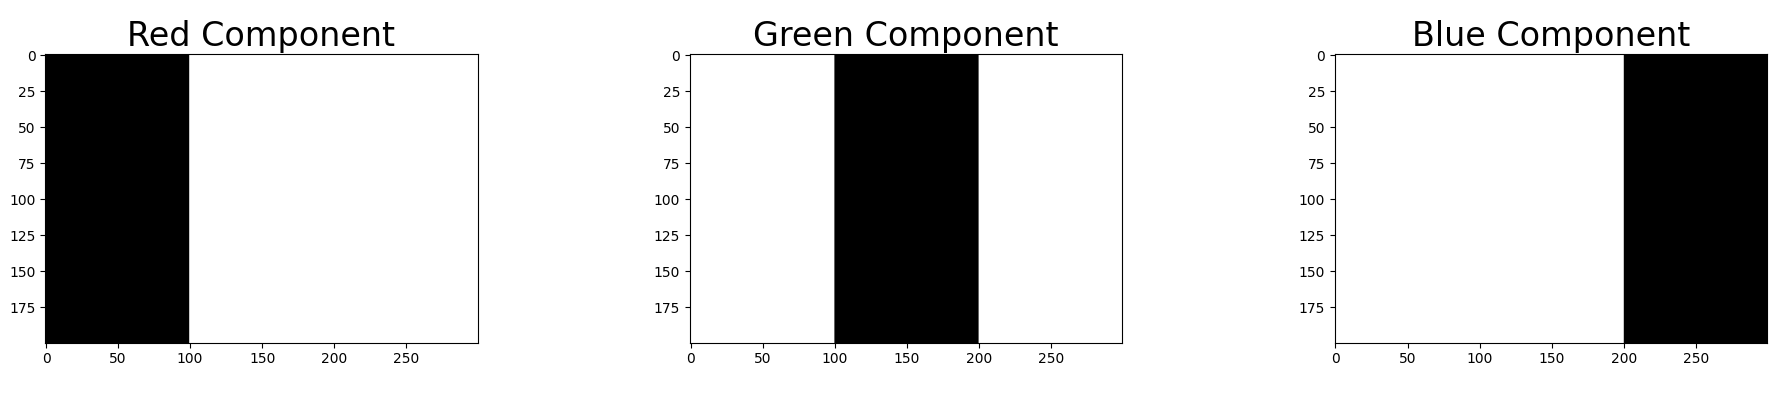
\includegraphics[scale=0.27]{test_image_rgb_plot.png}
		\caption{RGB Components of Test Image}
		\label{fig:test_image_rgb}
	\end{figure}

	Note that each component is now a greyscale image because each pixel is only taking values between 1 and 255 inclusively. 
	
	\section{Singular Value Decomposition (SVD)}
	We can represent our original image as three matrices of RGB components. On each of matrix, we can perform Singular Value Decomposition (SVD): 
	
	\begin{minted}[fontsize=\normalsize]{python}
# perform the SV decomposition
def __perform_svd(self, matrix: np.matrix) -> tuple:
	return np.linalg.svd(matrix)
	\end{minted}

	The code above wraps around a built in function from Pythons NumPy package. This has been done to integrate the functionality into a class object containing information about the image and a number of other methods. It takes a NumPy matrix object as its input and returns a tuple of three elements containing the $\textbf{U}\Sigma\textbf{V}^{\top}$ decomposition. The second element of the tuple is an ordered array containing the diagonal elements of $\Sigma$ to easily extract the singular values. We next need a function to retrieve the variance explained by a singular value:
	
	\begin{minted}[fontsize=\normalsize]{python}
# get the variance explained by the singular values
def var_singular(self, matrix: np.matrix, scale: bool = True) -> numpy.ndarray:
	if scale:
		matrix = self.__scale_matrix(matrix)
	matrix_U, matrix_s, matrix_V = self.__perform_svd(matrix)
	
	var_explained = np.round(matrix_s ** 2 / np.sum(matrix_s ** 2), decimals = 3)
	return var_explained
	\end{minted}
\end{document}